\documentclass{LabReport}
\title{操作系统实验报告}
\author{221900180 田永铭}
\date{\today}
\addbibresource{refs.bib}
\Chead{操作系统实验报告}
\Cfoot{\thepage}
\usepackage{listings}
\usepackage{graphicx} 

\begin{document}
	\maketitle
	\section{实验要求}
	使用nasm汇编编程实现一个MBR程序,每隔1秒钟左右输出一个(组)字符(自定),具体内容包括:\\
	1)实现一个时钟中断处理例程,按规定时间间隔输出字符(可使用BIOS提供的int 10h实现字符输出);\\
	2)修改中断向量表,将时钟中断处理例程起始地址填入中断向量表对应表项;\\
	3)设置8253/4定时器芯片,每隔20ms左右(自定 < 1秒)产生一次时钟中断
	\section{实验环境}
	
	\begin{itemize}
		\item 操作系统:Windows 11
		\item 编程语言:汇编
		\item 使用工具:qemu;vscode Hex Editor
		\item 虚拟系统版本:windows-7;linux-20-desktop
	\end{itemize}
	\section{实验原理}
	\textbf{时钟中断:}时钟中断是系统本身提供的重要中断服,8086系统还提供了可以给用户自定义修改的时钟中断。\par
	\hspace{0.1em}\textbf{修改中断向量表:}中断向量表是一个存储中断处理例程起始地址的表格。为了让系统在时钟中断发生时执行我们编写的中断处理例程,需要修改中断向量表,将时钟中断处理例程的起始地址填入对应的表项。\par
	\hspace{0.1em}\textbf{8253/8254定时器芯片:}这是一个可编程定时器芯片,通常用于在计算机中生成定时中断。在本实验中,可以设置8253/8254芯片,使其每隔约20毫秒产生一次时钟中断,以满足输出字符的要求。
	
	\section{实验过程}
	作业视频演示链接如下(上传至南大云盘,如果查看不了则需要{\color{red} 下载}查看)(作业附件中也有演示视频):\\
	\href{https://box.nju.edu.cn/f/d617483fc46f4cd98a7d/}{\color{red} 221900180\_田永铭\_实验3视频演示}\\
	
	实验主要分为以下几个步骤:
	
	\begin{enumerate}
		\item 修改中断向量表
		\item 设置8253/4定时器芯片
		\item 按规定时间间隔输出字符
		\item 整合代码
		\item 写入磁盘,查看运行效果
		\item 其他各种尝试和探索过程
	\end{enumerate}
	
	\subsection{修改中断向量表}
	参考\href{https://blog.csdn.net/nicholas199109/article/details/8557484?ops_request_misc=%257B%2522request%255Fid%2522%253A%2522171153468616800180615319%2522%252C%2522scm%2522%253A%252220140713.130102334.pc%255Fall.%2522%257D&request_id=171153468616800180615319&biz_id=0&utm_medium=distribute.pc_search_result.none-task-blog-2~all~first_rank_ecpm_v1~rank_v31_ecpm-2-8557484-null-null.142^v100^pc_search_result_base5&utm_term=8086%E6%97%B6%E9%92%9F%E4%B8%AD%E6%96%AD%E5%90%91%E9%87%8F%E8%A1%A8&spm=1018.2226.3001.4187}{\color{red} {8086中断向量表}},我们可以得到关键信息:定时器(IRQ0)的I/O地址为20h-23h,中断号为8h;同时,提供给用户的定时器控制的软中断,地址为70h-73h,中断号为1C。我们需要用到的是4*1C和4*1C+2的数字,即70h和72h,我们需要把中断服务程序入口地址偏移量存放到前者中,把中断服务程序入口地址的段基址放到后者中即可。
	\begin{lstlisting}[language=python,frame=shadowbox]
mov word [0x70], clock_handler ;修改中断,跳转clock_handler处理中断
mov word [0x72], 0

clock_handler:
;to do
	\end{lstlisting}
	
	
	\subsection{设置8253/4定时器芯片}
	为了让定时器每20ms就产生一个中断,我们需要修改定时器的频率,并且将计数值发送到计数器的端口。实现代码如下
	\begin{lstlisting}[language=python,frame=shadowbox]
; 设置定时器0(8253/8254)以产生时钟中断

; 发送命令字节到控制寄存器端口0x43
mov al, 00110110b ; 方式3,用于定时产生中断
out 0x43, al

; 计算计数值,产生20毫秒的时钟中断,时钟频率为1193180赫兹
; 计数值 = (时钟频率 / 每秒中断次数) - 1
; = (1193180 / (1 / 0.02)) - 1= 23863
mov ax, 23863

; 将计数值分为低字节和高字节,发送到计数器0的数据端口(端口0x40)
out 0x40, al        ; 低字节
mov al, ah
out 0x40, al        ; 高字节
	\end{lstlisting}
	
\subsection{按规定时间间隔输出字符}
定时器每20ms就产生一个中断,要想每1s输出一个字符,我们需要进行计数,每中断50次才打印。这里采用的是一个数据段,每次用cx从数据段中读计数,自增后写回,如果到了50,则打印并且重新计数,否则直接返回时钟中断。实现代码如下:
\begin{lstlisting}[language=python,frame=shadowbox]
lock_handler:
	;每次中断将数据段中值加1,加到50后才打印并且清零
	;实现1秒打印一次
	inc word [counter]
	mov cx, [counter]
	cmp cx, 50
	jne r
	mov si,msg
	call print
	mov word [counter], 0
	r:iret
	
exit:
	ret
	
print:
	; 打印字符
	lodsb
	or al, al
	jz exit
	mov ah, 0x0E
	int 0x10          ; 调用INT 10h中断
	jmp print
	
msg db "Yong-Ming Tian ", 0
\end{lstlisting}
	
	
	\subsection{整合代码}
	为了使得程序运行符合预期,我们还需要:
	\begin{enumerate}
		\item 整合代码,在代码开头设置起点,初始化
		\item 注意开始程序时用cli关中断,完成时钟设置后用sti开中断
		\item 在程序的最后添加jmp \$,使得程序不断运行
		\item 在代码最后填充剩余的512字节使得代码符合MBR要求
	\end{enumerate}
	完整代码如下:
	\begin{lstlisting}[language=python,frame=shadowbox]
BITS 16
SECTION MBR vstart=0x7c00

;稳妥使用栈
xor ax, ax
mov ds, ax
mov es, ax
mov ss, ax
mov cx, ax
mov sp, 0x7c00

counter dw 0x00;定义数据段

start:
	cli ;关中断
	
	;定时器提供的软中断地址是70-73,定时器地址是20-23
	mov word [0x70], clock_handler ;修改中断;
		;跳转clock_handler处理中断
	mov word [0x72], 0
	
	; 设置定时器0(8253/8254)以产生时钟中断
	
	; 发送命令字节到控制寄存器端口0x43
	mov al, 00110110b ; 方式3,用于定时产生中断
	out 0x43, al
	
	; 计算计数值,产生20毫秒的时钟中断,时钟频率为1193180赫兹
	; 计数值 = (时钟频率 / 每秒中断次数) - 1 
	;= (1193180 / (1 / 0.02)) - 1= 23863
	mov ax, 23863
	
	; 将计数值分为低字节和高字节,发送到计数器0的数据端口
	out 0x40, al        ; 低字节
	mov al, ah
	out 0x40, al        ; 高字节
	
	sti ;开中断
	jmp $   ;使程序不断停在这里执行等待时钟中断

; 时钟中断处理例程
clock_handler:
	;每次中断将数据段中值加1,加到50后才打印并且清零
	;实现1秒打印一次
	inc word [counter]
	mov cx, [counter]
	cmp cx, 50
	jne r
	mov si,msg
	call print
	mov word [counter], 0
	r:iret

exit:
	ret

print:
; 打印字符
	lodsb
	or al, al
	jz exit
	mov ah, 0x0E
	int 0x10          ; 调用INT 10h中断
	jmp print

msg db "Yong-Ming Tian ", 0

times 510-($-$$) db 0  ; 填充剩余的512字节以使文件大小为512字节
dw 0xAA55              ; MBR结束标志
	\end{lstlisting}
	

	\subsection{写入磁盘,查看运行效果}
	将asm文件编译并且写入磁盘,启动后查看效果,指令如下:\\
	\textbf{编译}(我的asm叫Timer.asm,编译生成的bin叫Timer.bin)
	\begin{lstlisting}[language=python,frame=shadowbox]
nasm -f bin Timer.asm -o Timer.bin
	\end{lstlisting}
	\textbf{写入虚拟磁盘}
	\begin{lstlisting}[language=python,frame=shadowbox]
dd if=Timer.bin of=os.img bs=512 count=1
	\end{lstlisting}
	{\bf 运行}
	\begin{lstlisting}[language=python,frame=shadowbox]
qemu-system-x86_64 -bios D:\MyOwnFiles\qemu\share\bios.bin -drive
file=os.img,format=raw -m 2G -smp 2
	\end{lstlisting}
	\textbf{查看运行效果:}在这一部分,我将通过视频详细展示我的代码运行结果,一共分为四部分:
	\begin{itemize}
		\item 设置时钟周期,使得20ms打印一次(速度中等)
		\item 设置时钟周期,使得45ms打印一次(速度慢)
		\item 设置时钟周期,使得2ms打印一次(速度快)
		\item 保持时钟周期20ms一次,实现50次中断打印一次(1s一次)
	\end{itemize}
	视频演示链接如下(上传至南大云盘,如果查看不了则需要{\color{red} 下载}查看)(作业附件中也有演示视频):\\
	\href{https://box.nju.edu.cn/f/d617483fc46f4cd98a7d/}{\color{red} 221900180\_田永铭\_实验3视频演示}\\
	同时,也展示一张图片简要展示结果:
	
\begin{figure}[h!]
	\centering
	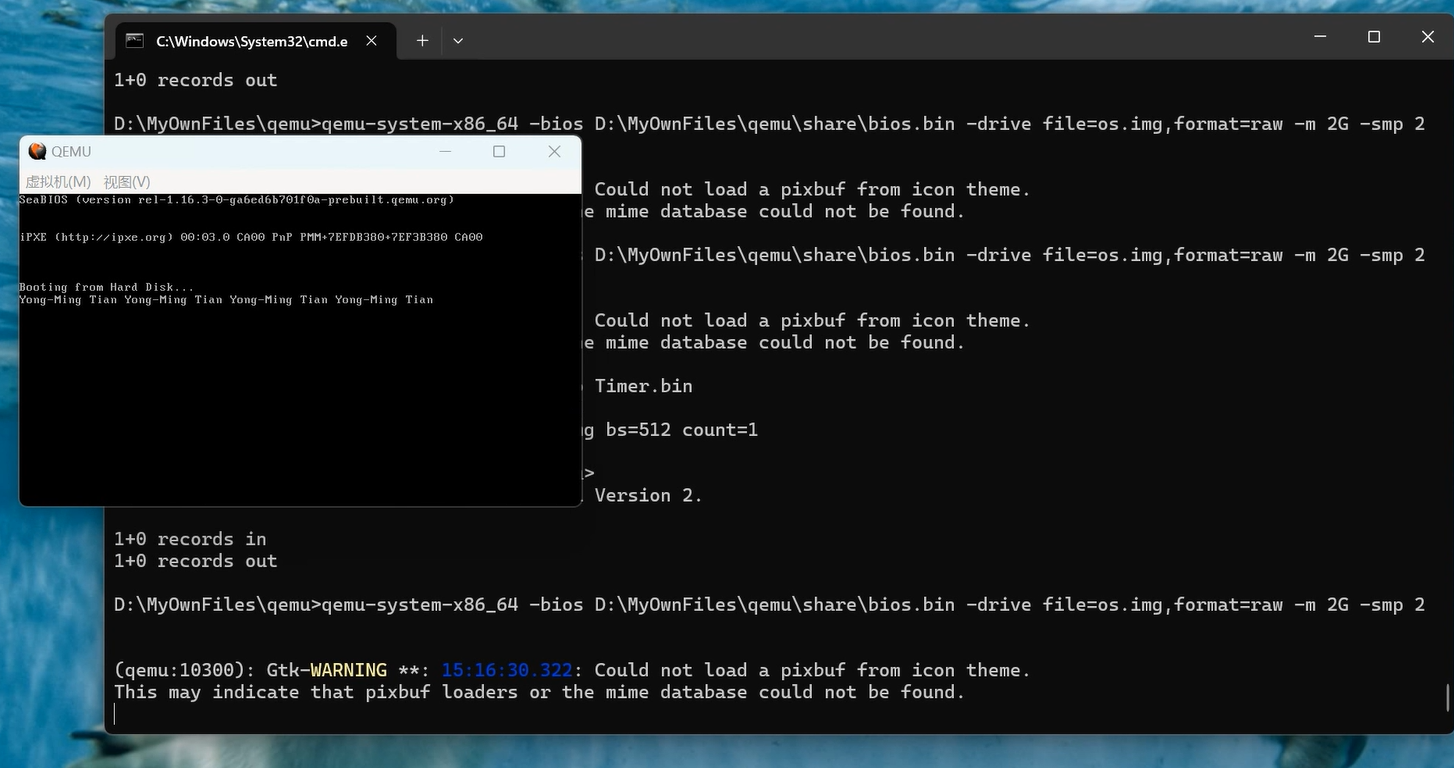
\includegraphics[width=\linewidth]{figures/1}
	\caption{打印Yong-Ming Tian}
	\label{fig:1}
\end{figure}
	
	
	\subsection{其他各种尝试和探索过程}
	在一开始实现计数50次中断打印一次字符的时候,我采用的时寄存器方法,但是失败了。那么利用寄存器能不能实现全局计数呢?\\
	\begin{lstlisting}[language=python,frame=shadowbox]
xor cx,cx
sti
jmp $

; 时钟中断处理例程
clock_handler:
	inc cx
	cmp cx, 50
	jne no_print
	mov si,msg
	call print
	iret
	\end{lstlisting}
以上代码显然是不合格的,在老师的帮助下,我进行了以下的思考:

	\subsubsection{防止print调用的int 10h修改cx的数值}
	在call print前后分别加上push cx,pop cx即可解决。但问题不在这。
	
	\subsubsection{考虑到中断也可能改变各种数值,需要更好的保存cx数值}
	\begin{lstlisting}[language=python,frame=shadowbox]
xor cx,cx
push 0

sti ;开中断
jmp $   ;使程序不断停在这里执行等待时钟中断

; 时钟中断处理例程
clock_handler:
pop cx
inc cx
push cx
cmp cx, 50
jne no_print
mov si,msg
call print
mov word [counter], 0
xor cx, cx
iret

no_print:
iret
	\end{lstlisting}
	
	
	\subsubsection{pop出的并非cx!}
	以上代码pop出来的不是cx,而是中断发生后,硬件压进去的最后一个寄存器值,比如flags,所以大部分情况是0。\par
	\hspace{0.5em}再次尝试在中断向量表的代码最后push cx,同时保存sp的值到bp,在中断处理程序中,直接用bp指向的内存位置读出值到cx,代码如下:
	\begin{lstlisting}[language=python,frame=shadowbox]
push cx
mov bp, sp
je print

sti ;开中断
jmp $   ;使程序不断停在这里执行等待时钟中断

; 时钟中断处理例程
clock_handler:
inc word [bp]
mov cx, [bp]
cmp cx, 50
jne no_print
mov si,msg
call print
mov word [counter], 0
xor cx, cx
mov word [bp], 0
iret
	\end{lstlisting}
	仍然不能实现实验要求。

	\subsubsection{原因分析}
	实际情况不会用通用寄存器去存放一个全局变量,存在一个内存单元中是常用的做法。这种非常规的做法可能会带来一系列问题:比如不能正确获取寄存器应该有的值,在虚拟机环境下中断发生后可能会修改一些重要的数值,这些对硬件知识的更多了解使得这种方法并不太可行。
	
	\subsubsection{其他拓展}
	除了时钟中断,我们还可以玩一玩别的中断,比如除0就会引发0号中断处理,我们采用相同的办法重写该中断程序,也能实现在其上打印字符。
	
	\section{实验结果}
	本人完全完成了本次实验的要求,并且在此基础上思考了其他实现方法的可能性,又对其他中断进行了新的把玩,收获颇丰。
	
	\section{总结与思考}
	\begin{itemize}
		\item 理论好理解不代表实验好做,实验需要非常多的细节,比如如何计数?利用寄存器来计数全局变量,显然不是一个好的选择
		\item STFW,RTFM 是计算机大类学生必备的素养,知识需要主动检索和学习
		\item 通过本次实验,我对中断向量表的理解更深了一步。在手写MBR的过程中,对时钟中断有了更直观的体验。尽管有些问题没有完全解决,但在解决问题过程中,我学到了更多的知识。
	\end{itemize}
	
	\section{其它参考文献}
	除了正文给出的参考文献,我参考的文献还有:\\\\
	\href{https://blog.csdn.net/qq_45931661/article/details/120576061?ops_request_misc=%257B%2522request%255Fid%2522%253A%2522171152047516800197016756%2522%252C%2522scm%2522%253A%252220140713.130102334..%2522%257D&request_id=171152047516800197016756&biz_id=0&utm_medium=distribute.pc_search_result.none-task-blog-2~all~baidu_landing_v2~default-1-120576061-null-null.142^v100^pc_search_result_base5&utm_term=%E4%BF%AE%E6%94%B9%E4%B8%AD%E6%96%AD%E5%90%91%E9%87%8F%E8%A1%A8&spm=1018.2226.3001.4187}{修改中断向量表}\\
	\hspace{2em}\href{https://blog.csdn.net/u011624903/article/details/121675034}{中断向量表0号中断}\\
	\href{https://blog.csdn.net/qq_61870465/article/details/134751137}{微机原理——定时器8253(8254)学习2应用与设计}\\
	\href{https://blog.csdn.net/qq_43645782/article/details/106339443?ops_request_misc=%257B%2522request%255Fid%2522%253A%2522171154013116800182726689%2522%252C%2522scm%2522%253A%252220140713.130102334.pc%255Fall.%2522%257D&request_id=171154013116800182726689&biz_id=0&utm_medium=distribute.pc_search_result.none-task-blog-2~all~first_rank_ecpm_v1~rank_v31_ecpm-15-106339443-null-null.142^v100^pc_search_result_base5&utm_term=%E6%B1%87%E7%BC%96%E5%88%A9%E7%94%A8%E6%97%B6%E9%92%9F8253%E4%B8%AD%E6%96%AD&spm=1018.2226.3001.4187}{用汇编实现8253定时计数器应用实验}\\
	\href{https://www.tutorialspoint.com/microprocessor/microprocessor_8086_interrupts.htm}{Microprocessor - 8086 Interrupts}
	
\end{document}